\documentclass[10pt]{beamer}

\usetheme[progressbar=frametitle]{metropolis}
\usepackage{appendixnumberbeamer}

\usepackage{subcaption}

\usepackage{booktabs}
\usepackage[scale=2]{ccicons}
\usepackage{tikz}
\usepackage{minted}
\usepackage{pgfplots}
\usepgfplotslibrary{dateplot}

\usepackage{xspace}
\newcommand{\themename}{\textbf{\textsc{metropolis}}\xspace}

\usepackage{polyglossia}
\setmainlanguage{spanish}


\definecolor{azul}{HTML}{B6E6FD}
\definecolor{rojo}{HTML}{FDAEAA}
\definecolor{amarillo}{HTML}{FFFFCA}

\title{Arquitectura Hexagonal}
\subtitle{Ejemplo práctico}
% \date{\today}
\date{}
\author{Luis Bertel}
\institute{}
% \titlegraphic{\hfill\includegraphics[height=1.5cm]{logo.pdf}}

\begin{document}

\maketitle

\begin{frame}{Tabla de contenido}
  \setbeamertemplate{section in toc}[sections numbered]
  \tableofcontents%[hideallsubsections]
\end{frame}

\section[Introducción]{Introducción}

\begin{frame}[fragile]{Introducción}
	
	La arquitectura hexagonal está basada en los principios de  \alert{Arquitecturas Limpias}. Éstas arquitecturas comparten un conjunto de buenas prácticas como lo son:
	
	\begin{itemize}
		\item Intependencia de los Frameworks.
		\item Testeable.		
		\item Independencia de la UI.
		\item Independencia de la persistencia de datos.
		\item Independencia de entidades externas.
	\end{itemize}

 
\end{frame}


\begin{frame}[fragile]{Capas de la arquitectura limpias}

\begin{figure}
	\centering
	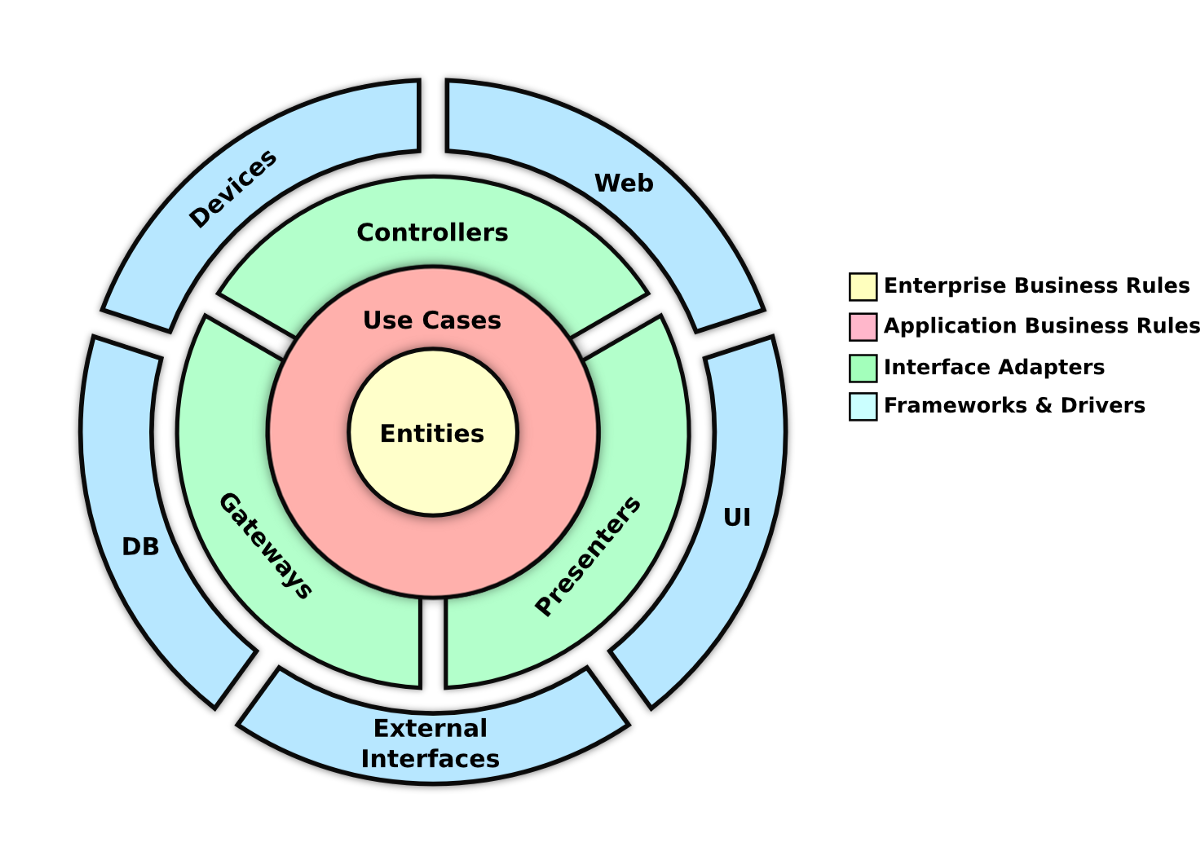
\includegraphics[width=0.8\linewidth]{img/JD606Sqx6RYZLKdu}
	\caption[clean]{Capas de arquitectura limpia}
	\label{fig:jd606sqx6ryzlkdu}
\end{figure}

\end{frame}

\begin{frame}[fragile]{Capas de la arquitectura hexagonal}
	
	\begin{figure}
		\centering
		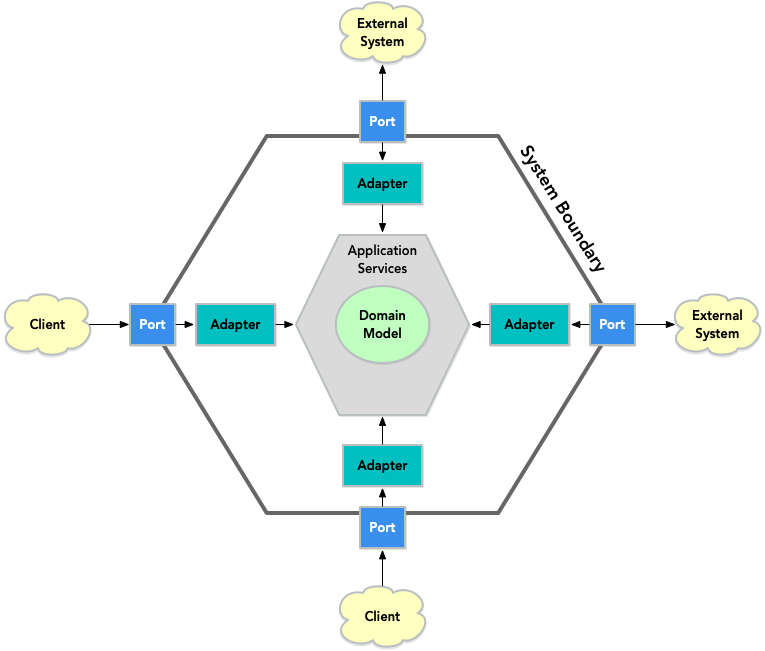
\includegraphics[width=0.7\linewidth]{img/hexagonal}
		\caption[clean]{Capas de arquitectura hexagonal}
		\label{fig:hexagonal}
	\end{figure}	
	
\end{frame}

\begin{frame}[fragile]{Capas de la arquitectura hexagonal}
	
\begin{figure}[h!]
	\centering
	\begin{subfigure}[b]{0.3\linewidth}
		% 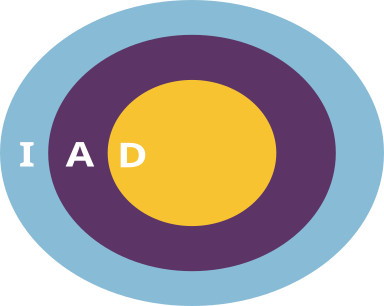
\includegraphics[width=\linewidth]{img/g4914}
		
		\begin{tikzpicture}
		% dibujo un círculo sin relleno
\draw[fill=azul] (0,0) circle (1.5cm);		
\draw[fill=rojo] (0,0) circle (1cm);
\draw[fill=amarillo] (0,0) circle (0.5cm);
	    
\draw
(0.0) node (d){D}
(-0.70,0) node (a) {A}
(-1.25,0) node (i){I};

		\end{tikzpicture}
				
		\caption{Vista de capas}
		\label{fig:vista_capas}
	\end{subfigure}
	\begin{subfigure}[b]{0.5\linewidth}
		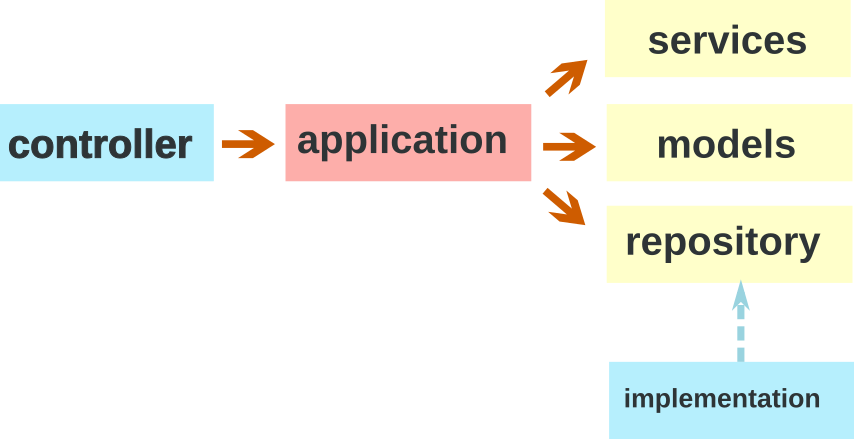
\includegraphics[width=\linewidth]{img/g12805}
		
		\caption{Vista desarrollo}
		\label{fig:vista_desarrollo}
	\end{subfigure}
	\caption{Modelo de capas de arquitectura hexagonal}
	\label{fig:arq_hexagonal}
\end{figure}
	
\end{frame}


\section{Caso de estudio}

\begin{frame}{Definición del cado de estudio}

Para nuestro ejemplo de estudio se implementará el caso de uso que recupera la información de una capacitación (\emph{training}) dado un identificador de tipo UUID (\emph{Universally Unique Identifier}). Si la capacitación con ese UUID no existe se retornará un valor de error 404 de tipo \emph{not found}. La persistencia se realizará en memoria. El ejercicio se realizará por iteraciones y la primera se enfocará en el flujo necesario para retornar la solicitud de la capacitación. Las demás iteraciones se enfocarán en el implementación utilizando la estructura DDD (\emph{Domain Drive Design}).

\end{frame}

\section{Infraestructura}

\begin{frame}{Infraestructura}

	La capa de infraestructura es el punto de entrada y salida con los demás sistemas. Además se encarga de aislar los elementos como frameworks, librerías, persistencias de vendors externos de las capas de aplicación y dominio.
	
	La capa de infraestructura implementa los adaptadores de la capa de dominio que sean necesarios para cumplir con los requerimientos del caso de uso (capa de aplicación).
		
\end{frame}

\begin{frame}[fragile]{Controller}

\begin{minted}[linenos,fontsize=\footnotesize,baselinestretch=1.0]{java}
@RestController
@RequestMapping("/api/formacion")
public final class TrainingByIdGetController {

    private final TrainingByIdHandler handler;

    public TrainingByIdGetController(TrainingByIdHandler handler){
        this.handler = handler;
    }

    @GetMapping("/training/{id}")
    public ResponseEntity<TrainingDTO> getTrainingById(@PathVariable UUID id){

        Optional<TrainingDTO> trainingDTO = this.handler.execute(id);

        if (trainingDTO.isPresent()){
             return new ResponseEntity(trainingDTO.get(), HttpStatus.OK);
        } else {
             return new ResponseEntity(new TrainingDTO(""), 
                   HttpStatus.NOT_FOUND);
        }
    }
}

\end{minted}


\end{frame}


\section{Aplicación}

\begin{frame}{Aplicación}

La capa de aplicación tiene la tarea de ejecutar la lógica de negocio y para ello puede utilizar servicios o repositorios. Los casos de usos pueden ser utilizados por más de un \alert{controlador}, \alert{eventbus} o cualquier \alert{input} del lado de infraestructura, incluso por otros casos de uso.

El caso de uso puede recibir valores primitivos, pero siempre va a retornar y a trabajar con Value Object.

\end{frame}


\begin{frame}[fragile]{Handler}

\begin{minted}[linenos,fontsize=\footnotesize,baselinestretch=1.0]{java}
@Component
public class TrainingByIdHandler {

    private final TrainingDAO dao;

    public TrainingByIdHandler(TrainingDAO dao) {
        this.dao = dao;
    }

    public Optional<TrainingDTO> execute(UUID id){
        return this.dao.getTrainingById(id);
    }
}
\end{minted}


\end{frame}

\section{Dominio}

\begin{frame}{Dominio}

En la capa de dominio contiene las clases de almacenamiento y entidades (contienen un UUID que permite identificarse) que modelan nuestro negocio. Las clases del dominio se diseñan para evitar el cambio de estado (no tienen set) y sus datos se asignan al momento de su creación por medio del constructor.

El dominio utiliza \alert{puertos} que permiten definir contratos de métodos que son implementados por la capa de infraestructura. Utilizando éste enfoque el dominio especifica el contrato e infraestructura los implementas. Un ejemplo contreto son los repositorio, el dominio define los datos que necesita para operar y la infraestructura realizar su implementación cumpliendo con el contrato ya sea utilizando una base de datos, eventbus, archivos planos, etc.

\end{frame}



\begin{frame}[fragile]{Data Transfer Object - DTO}

\begin{minted}[linenos,fontsize=\footnotesize,baselinestretch=1.0]{java}
public class TrainingDTO {

    private final String name;

    public TrainingDTO(String name) {
        this.name = name;
    }

    public String getName() {
        return name;
    }
}
\end{minted}

\end{frame}



\begin{frame}[fragile]{Data Access Object - DAO}

\begin{minted}[linenos,fontsize=\footnotesize,baselinestretch=1.0]{java}
public interface TrainingDAO {

    List<TrainingDTO> getAllTraining();
    Optional<TrainingDTO> getTrainingById(UUID id);

}
\end{minted}

\end{frame}


\begin{frame}[fragile]{Infraestructura - Implementación Repository}

\begin{minted}[linenos,fontsize=\footnotesize,baselinestretch=1.0]{java}
@Repository
public class InMemoryTrainingDAO implements TrainingDAO {

    @Override
    public List<TrainingDTO> getAllTraining() {

        List<TrainingDTO> dtos = new ArrayList<>();

        dtos.add(new TrainingDTO("Basic Java"));
        dtos.add(new TrainingDTO("Hexagonal Architecture"));
        dtos.add(new TrainingDTO("The importance of water in navigation"));
        dtos.add(new TrainingDTO("The super me in existential dilemmas"));

        return dtos;
    }

    @Override
    public Optional<TrainingDTO> getTrainingById(UUID id) {
   // esto hay que analizarlo mejor
        return Optional.ofNullable(
            new TrainingDTO("The super me existential dilemmas"));
    }
}
\end{minted}


\end{frame}

\section{Docker}

\begin{frame}[fragile]{Comandos de docker}

\alert{Descarga de una imagen}

\mint{bash}|> docker pull ubuntu|

\alert{Listado de imagenes descargadas}

\mint{bash}|> docker images|

\begin{minted}[fontsize=\footnotesize,baselinestretch=1.0]{bash}
REPOSITORY                    TAG                     IMAGE ID            CREATED             SIZE
maestro-server                v1.0                    a7df52488e71        7 days ago          676MB
redis                         6.0-alpine3.11          0b4e853530a5        7 days ago          31.6MB
rabbitmq                      3.8-management-alpine   a6ce06daac72        8 days ago          139MB
mysql/mysql-server            latest                  671b2c453d03        8 days ago          139MB
formacion-server              v1.0                    d4f8885f07ee        8 days ago          701MB
gateway-server                v1.0                    3f0b5eba91c9        8 days ago          671MB
eureka-server                 v1.0                    8e2215c019d9        8 days ago          685MB
redis                         <none>                  360360313017        2 weeks ago         31.6MB
rabbitmq                      <none>                  e64c67658b55        2 weeks ago         139MB
mysql/mysql-server            <none>                  716286be47c6        2 weeks ago         381MB
openjdk                       11                      f5de33dc9079        3 weeks ago         627MB
parrotstream/centos-openjdk   latest                  59dbb5986f22        19 months ago       920MB
\end{minted}


\end{frame}


\begin{frame}[fragile]{Comandos de docker}

\alert{Listado de imágenes ejecutandose}

\mint{bash}|> docker ps -a|

\alert{Listado de imágenes ejecutandose -otra forma-}

\mint{bash}|> docker ps --format "table {{.ID}}\t{{.Names}}"|

\begin{minted}[fontsize=\footnotesize,baselinestretch=1.0]{bash}
CONTAINER ID        NAMES
784b92cf40bc        eureka-server
6a110c9f8e9e        gateway-server
3d5f53436e9a        maestro-server
5f4bdc9e48ec        rabbitmq-server
e30d1d74928d        redis-server
\end{minted}


\end{frame}


\begin{frame}[fragile]{Comandos de docker}

\alert{Detener una imagen}

\mint{bash}|> docker stop redis-server|

\alert{Eliminar una imagen -debe estar detenida-}

\mint{bash}|> docker rm redis-server|

\alert{Correr una imagen}

\begin{minted}[fontsize=\footnotesize,baselinestretch=1.0]{bash}
> docker run -p 6379:6379 --name redis-server --restart always 
       -d redis:6.0-alpine3.11
b519b42a60f7973de76dc8395af2e9b84753d21b0043e9c9779f76c78dcb7dec
\end{minted}

\end{frame}


\begin{frame}[fragile]{Anatomia de un Dockerfile}


\begin{minted}[linenos, fontsize=\footnotesize,baselinestretch=1.0]{docker}
FROM openjdk:11

MAINTAINER "Luis Bertel" lbertel@gmail.com

RUN mkdir /app
ADD ./build/libs/formacion-server-1.0.jar /app/formacion-server-1.0.jar
ENTRYPOINT ["java","-jar","/app/formacion-server-1.0.jar"]
\end{minted}

\alert{Ejecutar el Dockerfile}

\mint{bash}|> docker build -t formacion-server .|

\emph{Se debe estar ubicado en el mismo directorio donde esta el Dockerfile y 
no olvide el punto al final del comando}.

\end{frame}


\section{Pendientes}

\begin{frame}[fragile]{Pendientes}

\begin{enumerate}
	\item Domain Drive Design
	\begin{enumerate}
		\item Implementación de Value Object
		\item Aggregate y aggregate root
		\item Command para los casos de usos
	\end{enumerate}
	\item Test
		\begin{enumerate}
		\item Unitarios
		\item Aceptación
		\item Integración
	\end{enumerate}		
\end{enumerate}

No olviden los principios de los patrones SOLID y STUPID.

\end{frame}


\end{document}